\chapter{APPENDIX}
\section{Crap for me}

\subsection{Local Gauge Transformation}
Free Dirac Equation:
\begin{equation*}
\Lagr_{\text{free}}(x) = \overline{\Psi}(x)(i\gamma^{\mu}\partial_{\mu}-m)\Psi(x),
\end{equation*}
Local Gauge Transformation:
\begin{equation*}
\Psi(x) \to e^{iq\chi(x)}\Psi(x),
\end{equation*}
Apply:
\begin{equation*}
\Lagr_{\text{free}} = e^{-iq\chi}\overline{\Psi}(i\gamma^{\mu}\partial_{\mu}-m)e^{iq\chi}\Psi
\end{equation*}
Expand:
\begin{equation*}
\Lagr_{\text{free}} = i\gamma^{\mu}.e^{-iq\chi}\overline{\Psi}\partial_{\mu}(e^{iq\chi}\Psi)-m.e^{-iq\chi}.e^{iq\chi}\overline{\Psi}\Psi
\end{equation*}
\begin{equation*}
\Lagr_{\text{free}} = i\gamma^{\mu}.e^{-iq\chi}\overline{\Psi}(e^{iq\chi}\partial_{\mu}\Psi+\partial_{\mu}(e^{iq\chi})\Psi)-m\overline{\Psi}\Psi
\end{equation*}
\begin{equation*}
\Lagr_{\text{free}} = i\gamma^{\mu}\overline{\Psi}\partial_{\mu}\Psi+i\gamma^{\mu}.e^{-iq\chi}.\overline{\Psi}.iq\partial_{\mu}\chi.e^{iq\chi}.\Psi)-m\overline{\Psi}\Psi
\end{equation*}
Final:
\begin{equation*}
\Lagr_{\text{free}} = \Lagr_{\text{free}}-q\gamma^{\mu}.\overline{\Psi}.\partial_{\mu}\chi.\Psi
\end{equation*}

\subsection{Local gauge principle} % (fold)
\label{sub:local_gauge_principle}

Add in additional field to Dirac equation*:
\begin{equation*}
i\gamma^{\mu}(\partial_{\mu}+iqA_{\mu})\Psi(x)-m\Psi(x)=0
\end{equation*}
Local Gauge Transformation:
\begin{equation*}
\Psi(x) \to e^{iq\chi(x)}\Psi(x)
\end{equation*}
Apply:
\begin{equation*}
i\gamma^{\mu}(\partial_{\mu}+iqA_{\mu})e^{iq\chi}\Psi-m.e^{iq\chi}\Psi=0
\end{equation*}
\begin{equation*}
i\gamma^{\mu}.\partial_{\mu}(e^{iq\chi}\Psi)+i\gamma^{\mu}.iqA_{\mu}.e^{iq\chi}\Psi-m.e^{iq\chi}\Psi=0
\end{equation*}
\begin{equation*}
i\gamma^{\mu}.e^{iq\chi}.\partial_{\mu}\Psi+i\gamma^{\mu}.iq\partial_{\mu}\chi e^{iq\chi}\Psi-q\gamma^{\mu}.A_{\mu}.e^{iq\chi}\Psi-m.e^{iq\chi}\Psi=0
\end{equation*}
\begin{equation*}
\text{Dirac}_\text{free}-q\gamma^{\mu}\partial_{\mu}\chi\Psi-q\gamma^{\mu}.A_{\mu}\Psi=0
\end{equation*}
To maintain invariance the local gauge transformation of $A_{\mu}$ must go as:
\begin{equation*}
A_{\mu} \to A_{\mu} - \partial_{\mu}\chi
\end{equation*}
So:
\begin{equation*}
\text{Dirac}_\text{free}-q\gamma^{\mu}\partial_{\mu}\chi\Psi-q\gamma^{\mu}.A_{\mu}\Psi+q\gamma^{\mu}.\partial_{\mu}\chi\Psi=0
\end{equation*}
\begin{equation*}
=\text{Dirac}_\text{int}
\end{equation*}
This new field exhibits the observed gauge invariance of classical electromagentism.
% subsection local_gauge_principle (end)

\subsection{Dirac Equation from Lagrangian} % (fold)
\label{sub:dirac_equation*_from_lagrangian}

Lagrangian Density for Dirac Field
\begin{equation*}
\Lagr = i\overline{\Psi}\gamma^{\mu}\partial_{\mu}\Psi-m\overline{\Psi}\Psi,
\end{equation*}
E-L equation
\begin{equation*}
\frac{\partial \Lagr}{\partial \Psi} - \frac{\partial}{\partial x^{\mu}} \left[\frac{\partial \Lagr}{\partial(\partial_{\mu}\Psi)}\right] = 0 
\end{equation*}
\begin{equation*}
\frac{\partial \Lagr}{\partial \overline{\Psi}} - \frac{\partial}{\partial x^{\mu}} \left[\frac{\partial \Lagr}{\partial(\partial_{\mu}\overline{\Psi})}\right] = 0
\end{equation*}
Sub
\begin{equation*}
i\gamma^{\mu}\partial_{\mu}\Psi-m\Psi-\frac{\partial}{\partial x^{\mu}}[0]
\end{equation*}
Dirac equation of motion
\begin{equation*}
i\gamma^{\mu}\partial_{\mu}\Psi-m\Psi
\end{equation*}
% subsection dirac_equation*_from_lagrangian (end)


\subsection{Free particle solution to Dirac Equation} % (fold)
\label{sub:free_particle_solution_to_dirac_equation*}
\begin{equation*}
	\Psi_{u} = u(p)e^{i(\mathbf{p.x}-E.t)}\,\,\text{and}\,\,\Psi_{v} = v(p)e^{-i(\mathbf{p.x}-E.t)}
\end{equation*}
% subsection free_particle_solution_to_dirac_equation* (end)



\subsection{Pauli spin matrices} % (fold)
\label{sub:pauli_spin_matrices}
\begin{equation*}
\sigma_{1} = 
\begin{pmatrix} 
	0 	& 	1 \\
	1 	& 	0 \\
\end{pmatrix}
\sigma_{2} = 
\begin{pmatrix} 
	0 	& 	-i \\
	i 	& 	0 \\
\end{pmatrix}
\sigma_{3} = 
\begin{pmatrix} 
	1 	& 	0 \\
	0 	& 	-1 \\
\end{pmatrix}
\end{equation*}
% subsection pauli_spin_matrices (end)


\subsection{Gamma matrices and relations} % (fold)
\label{sub:gamma_matrices_and_relations}

\begin{equation*}
\gamma^{0} = 
\begin{pmatrix} 
	1 	& 	0	&	0	&	0 \\
	0 	& 	1	&	0	&	0 \\
	0 	& 	0	&	-1	&	0 \\
	0 	& 	0	&	0	&	-1 \\
\end{pmatrix}
\gamma^{1} = 
\begin{pmatrix} 
	0 	& 	0	&	0	&	1 \\
	0 	& 	0	&	1	&	0 \\
	0 	& 	-1	&	0	&	0 \\
	-1 	& 	0	&	0	&	0 \\
\end{pmatrix}
\end{equation*}

\begin{equation*}
\gamma^{2} = 
\begin{pmatrix} 
	0 	& 	0	&	0	&	-i \\
	0 	& 	0	&	i	&	0 \\
	0 	& 	i	&	0	&	0 \\
	-i 	& 	0	&	0	&	0 \\
\end{pmatrix}
\gamma^{3} = 
\begin{pmatrix} 
	0 	& 	0	&	1	&	0 \\
	0 	& 	0	&	0	&	-1 \\
	-1 	& 	0	&	0	&	0 \\
	0 	& 	1	&	0	&	0 \\
\end{pmatrix}
\end{equation*}

\begin{equation*}
	(\gamma^{0})^{2} = I
\end{equation*}
\begin{equation*}
	(\gamma^{k})^{2} = -I
\end{equation*}
\begin{equation*}
	\gamma^{0\dagger} = \gamma^{0}
\end{equation*}
\begin{equation*}
	\gamma^{k\dagger} = -\gamma^{k}
\end{equation*}
\begin{equation*}
	[\gamma^{\mu}, \gamma^{\nu}] = \gamma^{\mu}\gamma^{\nu}+\gamma^{\nu}\gamma^{\mu} = 2g^{\mu\nu}
\end{equation*}

\begin{equation*}
	\gamma^{5} = i\gamma^{0}\gamma^{1}\gamma^{2}\gamma^{3}
\begin{pmatrix} 
	0 	& 	0	&	1	&	0 \\
	0 	& 	0	&	0	&	1 \\
	1 	& 	0	&	0	&	0 \\
	0 	& 	1	&	0	&	0 \\
\end{pmatrix}
\end{equation*}
\begin{equation*}
	(\gamma^{5})^{2} = 1
\end{equation*}
\begin{equation*}
	\gamma^{5\dagger} = \gamma^{5}
\end{equation*}
\begin{equation*}
	[\gamma^{5}, \gamma^{\mu}] = -\gamma^{\mu}\gamma^{5}
\end{equation*}
% subsection gamma_matrices (end)


\subsection{Gellman matrices} % (fold)
\label{sub:gellman_matrices}
\begin{equation*}
	\lambda^{1} = 
\begin{pmatrix} 
	0 	& 	1	&	0 \\
	1 	& 	0	&	0 \\
	0 	& 	0	&	0 \\
\end{pmatrix}
	\lambda^{2} = 
\begin{pmatrix} 
	0 	& 	-i	&	0 \\
	i 	& 	0	&	0 \\
	0 	& 	0	&	0 \\
\end{pmatrix}
	\lambda^{3} = 
\begin{pmatrix} 
	1 	& 	0	&	0 \\
	0 	& 	-1	&	0 \\
	0 	& 	0	&	0 \\
\end{pmatrix}
\end{equation*}

\begin{equation*}
	\lambda^{4} = 
\begin{pmatrix} 
	0 	& 	0	&	1 \\
	0 	& 	0	&	0 \\
	1 	& 	0	&	0 \\
\end{pmatrix}
	\lambda^{5} = 
\begin{pmatrix} 
	0 	& 	0	&	-i \\
	0 	& 	0	&	0 \\
	i 	& 	0	&	0 \\
\end{pmatrix}
	\lambda^{6} = 
\begin{pmatrix} 
	0 	& 	0	&	0 \\
	0 	& 	0	&	1 \\
	0 	& 	1	&	0 \\
\end{pmatrix}
\end{equation*}

\begin{equation*}
	\lambda^{7} = 
\begin{pmatrix} 
	0 	& 	0	&	0 \\
	0 	& 	0	&	-i \\
	0 	& 	i	&	0 \\
\end{pmatrix}
	\lambda^{8} = \frac{1}{\sqrt{3}}
\begin{pmatrix} 
	1 	& 	0	&	0 \\
	0 	& 	1	&	0 \\
	0 	& 	0	&	2 \\
\end{pmatrix}
\end{equation*}
% subsection gellman_matrices (end)


\subsection{Symmetry breaking} % (fold)
\label{sub:symmetry_breaking}
Consider scalar potential:
\begin{equation*}
	V(\phi) = \frac{1}{2}\mu^{2}\phi^{2} + \frac{1}{4}\lambda\phi^{4}
\end{equation*}
The corresponding lagrangian is given by:
\begin{equation*}
	\Lagr = T - V
\end{equation*}
\begin{equation*}
	\Lagr = \frac{1}{2}(\partial_{\mu}\phi)(\partial^{\mu}\phi) - \frac{1}{2}\mu^{2}\phi^{2} - \frac{1}{4}\lambda\phi^{4}
\end{equation*}
where $(\partial_{\mu}\phi)(\partial^{\mu}\phi)$ is the kinematic term for a scalar particle, $\mu^{2}\phi^{2}$ represents the mass term and $\lambda\phi^{4}$ term represents the self interactions of the scalar field.

The vacuum state is the lowest energy state of $\phi$ which corresponds to a minimum of $V(\phi)$. For $\phi$ to generate a minimum $\lambda>0$, however there are no such restrictions on $\mu^{2}$.
\begin{figure}[htpb]
	\centering
	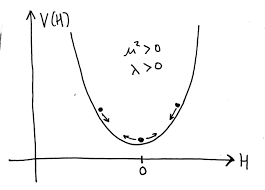
\includegraphics[width=0.24\textwidth]{Figures/hpot1}
	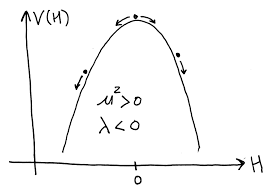
\includegraphics[width=0.24\textwidth]{Figures/hpot2}
	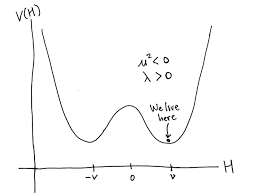
\includegraphics[width=0.24\textwidth]{Figures/hpot3}
	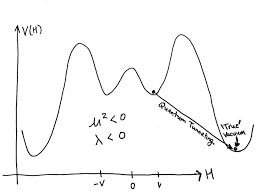
\includegraphics[width=0.24\textwidth]{Figures/hpot4}
\end{figure}
If $\mu^{2}>0$, this result in a scalar particle of mass $\mu$ with self interaction $\propto\phi^{4}$
If $\mu^{2}<0$, $\mu$ is no longer interpretated as a mass. The minimum of $\phi$ occurs at degenerate $\pm v = \pm \left|\sqrt{\frac{-\mu^2}{\lambda}}\right|$, which leads to 
\begin{equation*}
	-\lambda v^2 = \mu^2
\end{equation*}
The choice of $+v$ or $-v$, breaks the symmetry of the lagrangian. This is spontaneous symmetry breaking.
Choosing vacuum state of field to be at $+v$, the excitations of the field (decribing particle states) can be obtained through perturbation theory
\begin{equation*}
	\phi(x)\to v + \eta(x), \,\,\,\, \partial_{\mu}\phi = \partial_{\mu}\eta
\end{equation*}
The lagrangian becomes
\begin{equation*}
	\Lagr = \frac{1}{2}(\partial_{\mu}\eta)(\partial^{\mu}\eta) - \frac{1}{2}\mu^{2}(v+\eta)^{2} - \frac{1}{4}\lambda(v+\eta)^{4}
\end{equation*}
\begin{equation*}
	\Lagr = \frac{1}{2}(\partial_{\mu}\eta)(\partial^{\mu}\eta) - \lambda v^2\eta^2 - \lambda v\eta^3 - \frac{1}{4}\lambda \eta^4 + \frac{1}{4}\lambda v^4 
\end{equation*}
The term $\propto\eta^2$ is interpretated as a mass. ($\eta$ is a massive scalar field) $m_{\eta} = \sqrt{2\lambda v^2}$.
Terms term $\propto\eta^3$ and term $\propto\eta^4$ are triple and quartic couplings of the field.
Thios lagrangian is essentially the same as the initial except with excitations perturbed about a non-zero vacuum expectation value
% subsection symmetry_breaking (end)

\subsection{The full standard model} % (fold)
\label{sub:the_full_standard_model}
\begin{equation*}
	\Lagr_{\SM} = \Lagr_{\QCD} + \Lagr_{\EWK} + \Lagr_{\mathrm{H}} + \Lagr_{\mathrm{Y}}
\end{equation*}
\begin{equation*}
	\Lagr_{\QCD}=\overline{\Psi}_{i}(i(\gamma^{\mu}D_{\mu})_{ij}-m\delta_{ij})\Psi_{j} - \frac{1}{4}G^{\mu \nu}_{a}G^{a}_{\mu \nu},
\end{equation*}
\begin{equation*}
\Lagr_{\EWK}=\overline{\Psi}i\gamma^{\mu}D_{\mu}\Psi - \frac{1}{4}B^{\mu\nu}B_{\mu\nu} - \frac{1}{4}W^{\mu\nu}_{i}W_{\mu\nu}^{i},
\end{equation*}
\begin{equation*}
	\Lagr_{\mathrm{H}}=(D_{\mu}\phi)^{\dagger}(D^{\mu}\phi)-\frac{1}{2}\mu^{2}\phi^{\dagger}\phi - \frac{1}{4}\lambda(\phi^{\dagger}\phi)^{2}
\end{equation*}
\begin{equation*}
	\Lagr_{\mathrm{Y}} = g_{y}\overline{\Psi}_{\mathrm{R}}\phi\Psi_{\mathrm{L}}, 
\end{equation*}
% subsection the_full_standard_model (end)

\subsection{DEBUG:NOETHER} % (fold)
\label{sub:tmp_noether}
e.g. m in orbit
\begin{equation*}
	L = \frac{1}{2}mv^{2} + \frac{GMm}{r}
\end{equation*}
and in polar coordinates:
\begin{equation*}
	L = \frac{1}{2}m\dot{r}^{2} + \frac{1}{2}mr^{2}\dot{\phi}^{2} + \frac{GMm}{r}
\end{equation*}
This equation* of motion is independent of $\phi$ and therefore angularly invariant.
The Euler-Lagrange Equation is:  
\begin{equation*}
	\frac{d}{dt}\left(\frac{\partial L}{\partial\dot{\phi}}\right) - \frac{\partial L}{d\phi}  = 0
\end{equation*}
The conserved current:
\begin{equation*}
	J = \frac{\partial L}{\partial\dot{\phi}} = mr^{2}\dot{\phi}
\end{equation*}
\begin{equation*}
	\frac{dJ}{dt} = \frac{1}{2}r\ddot{\phi} + \dot{r}\dot{\phi} = 0
\end{equation*}
This is equivalent to the conservation of angular momentum

